% this file is called up by thesis.tex
% content in this file will be fed into the main document
\chapter{Knowledge Based Design} % top level followed by section, subsection
%: ----------------------- paths to graphics ------------------------

% change according to folder and file names
\ifpdf
    \graphicspath{{2.5/figures/PNG/}{2.5/figures/PDF/}{2.5/figures/}}
\else
    \graphicspath{{2.5/figures/EPS/}{2.5/figures/}}
\fi

%: ----------------------- contents from here ------------------------

\section{Knowledge based Design (KBD)}
Knowledge based Design can be classified as a Knowledge-based system (KBS), systems based on the methods and techniques of Artificial Intelligence. Their core components are the knowledge base and inference mechanisms. In this thesis a KBS that resembles Case-Based Reasoning (CBR) is combined with EAs, in an optimal way, giving rise to the proposed KBD method. CBR can be seen as a problem solving method that 
reuses past cases and experience to conceive a solution to a current problem. 
While other major artificial intelligence techniques rely on mapping generalized 
relationships between problem descriptions and conclusions. CBR has the benefit 
of utilizing previous experience based on concrete old-problem solutions. 
The central tasks of a CBR system to identify the problem in hand find one or 
more similar past case(s), use this information to suggest a solution to the current 
problem and update the system by learning from this experience \cite{kolodner_1991,kolodner_1993,slade_1991,riesbeck_1989}.      
%***********************************************************************

\paragraph{Historic note}
%***********************************************************************
\label{History} It is widely held that the origins of CBR lays in the work of 
Schank and Abelson in 1977 \cite{Schank_Abelson_1977}. They proposed that general 
human knowledge about situations is recorded as scripts that allows the extract 
of expectations and inferences. Scripts were proposed as structure for conceptual 
memory describing information about stereotypical events. However, experiments 
showed that they are not a complete theory of memory representation -people 
often confuse events with similar scripts. Such observations fell in line with 
concept formulation, problem solving and experimental learning theories within 
philosophy and psychology \cite{tulving_1977,smith_1978}. 

Roger Schank continued to investigate the role of previews situations (i.e. cases) 
and situation patterns role in both problem solving and learning \cite{Schank_1982}. 
Simultaneously Gentner \cite{genter_1983} was developing a also relevant to CBR 
theoretical framework for analogy. Significant references to CBR can also be fount in 
Wittgensteins's observation \cite{wittgestein_1953} that natural concepts are in fact 
polymorphic and can not be classified by a single set of necessary and sufficient 
features but instead can be defined by a set of instances (i.e. cases) with family 
resemblances. This work has been cited as the philosophical basis for CBR by Aamondt and Plaza \cite{aamond_plaza_1994}.

Even though the "philosophical" roots of CBR could be claimed by many, it was Roger Schank and his group that in the early eighties produced both a cognitive model and the first CBR applications based on it. Janet Kolonder developed the first CBR system called CYRUS \cite{kolodner_1983a,kolodner_1983b} which was an implementation of Schank's dynamic memory model. Its case-memory model later served as the basis for several other CBR systems. Spreading there use in a lot of disciplines raging from law \cite{ashley_1988,rissland_skalak_1989} to civil engineering \cite{whatson_abdullah_1994,moore_1994}

%***********************************************************************
\subsection{Case-Based Reasoning}
%***********************************************************************
\label {CBR}  The classic definition of CBR was coined by Riesbeck and Schank \cite{riesbeck_1989}:

"A case-based reasoner solves problems by using or adapting solutions to old problems". 
Which answers exactly the what a CBR system should do but not the how it dose it. The answer 
to the second question is commonly described by the so called CBR-cycle (Fegure 1). 
%-----------------------------------------------------------------------
\paragraph{CBR Cycle}
%-----------------------------------------------------------------------
\label{CBR Cycle} CBR is based on four logical steps described by Aamodt and Plaza 
\cite{aamond_plaza_1994} as a typical cyclical process comprising the four REs: 

\begin{itemize}
  \item RETRIEVE the most similar case(s);
  \item REUSE the case(s) to attempt to solve the problem;
  \item REVISE the proposed solution if necessary, and
  \item RETAIN the new solution in the Case-Base.
\end{itemize}
which can be represented by a schematic cycle (see Figure \ref{cbr}).

\figuremacroW{cbr}{CBR}{Schematic cycle representing the four REs}{0.5}

%\begin{center}
%\begin{tabular}{ c }
%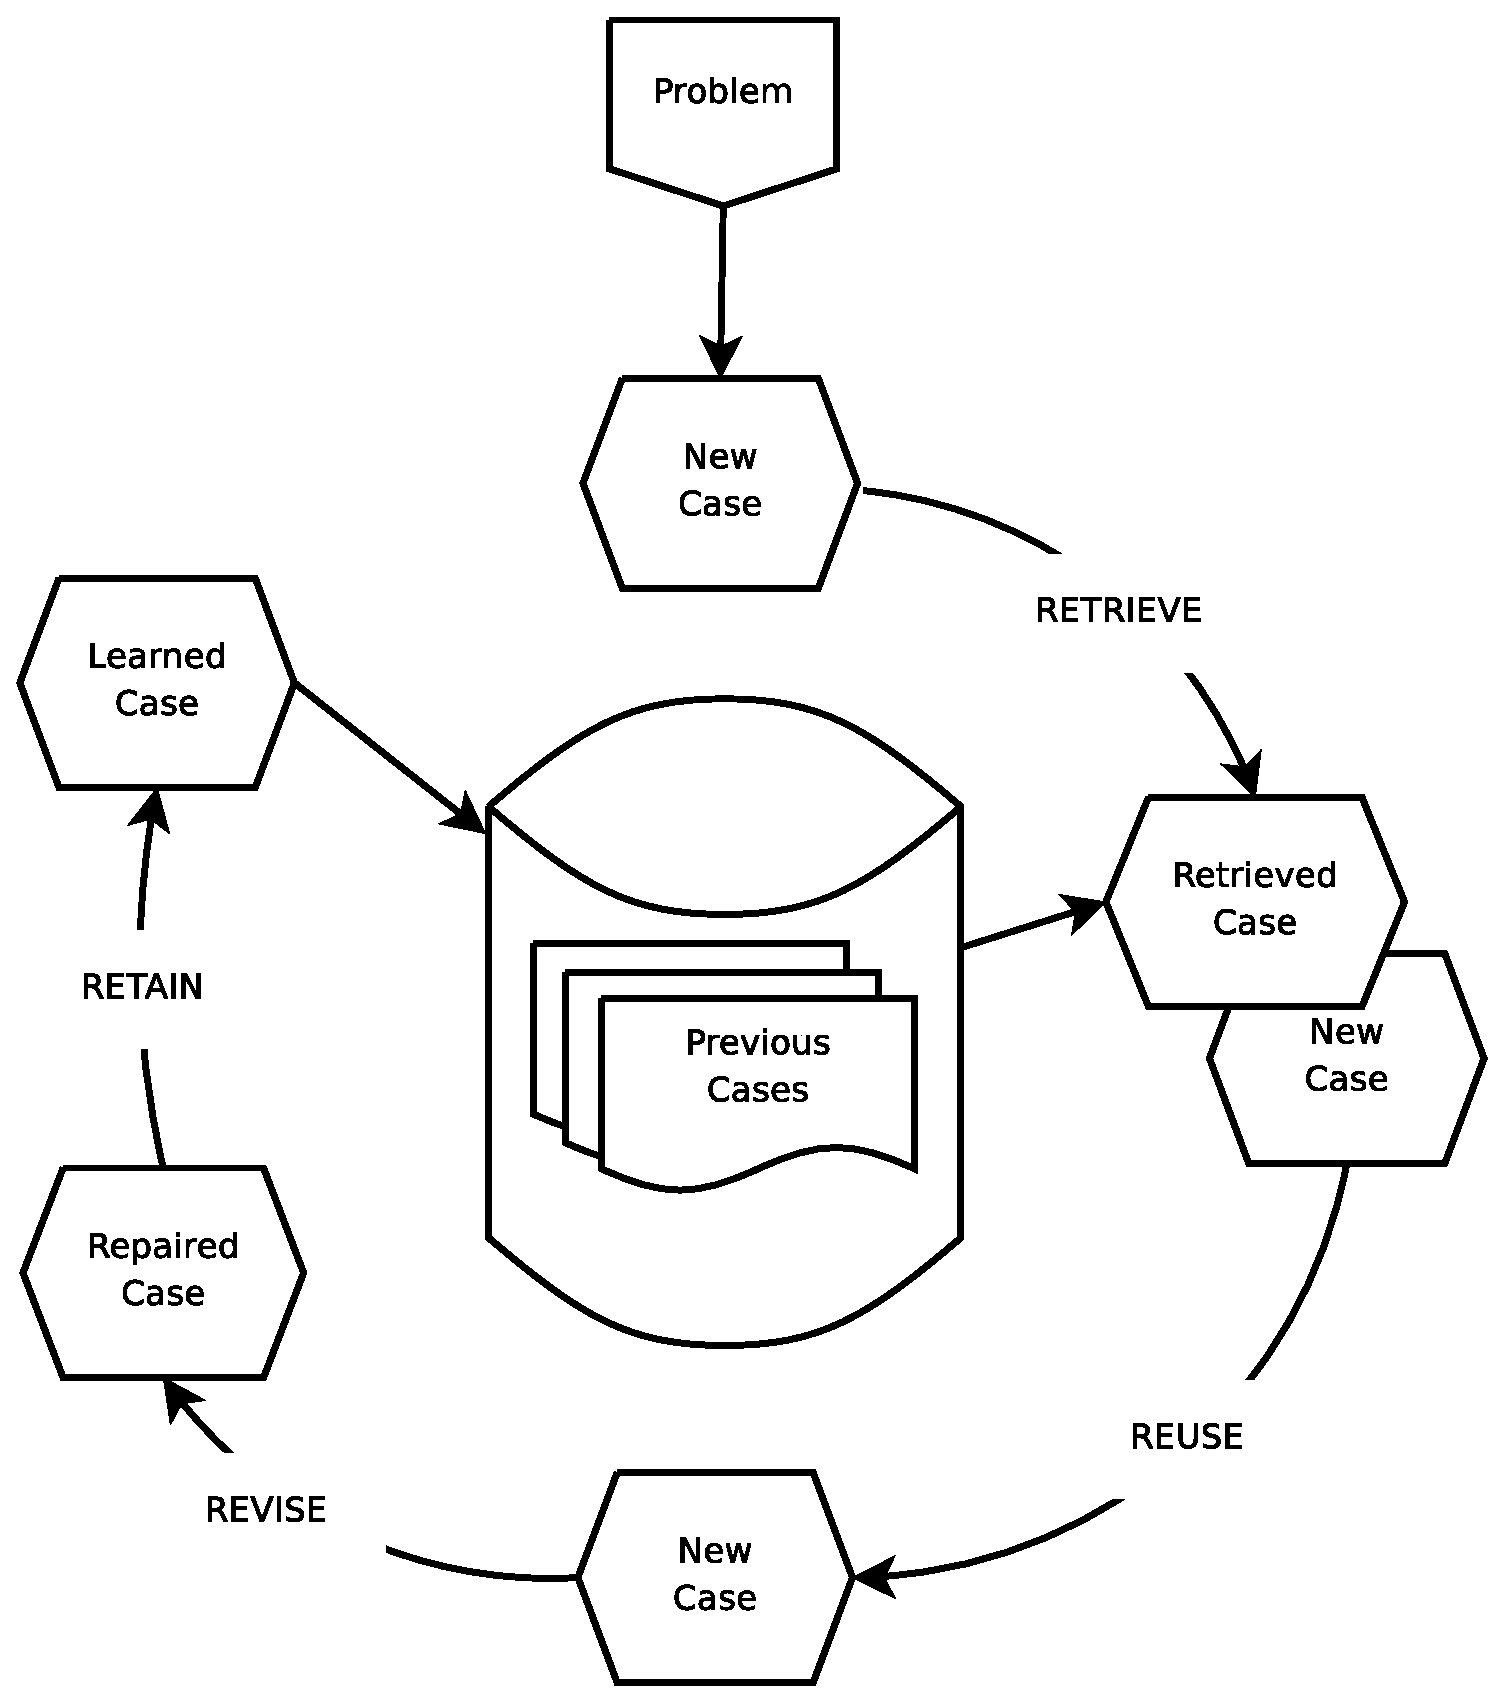
\includegraphics[width=70mm]{cbr.eps} \\
%Figure 1 Schematic cycle representing the four REs.
%\end{tabular}
%\end{center}

A new problem is matched against cases in the case base and thought a similarity 
criterion one or more similar cases are retrieved. A solution is suggested by the 
matching cases. Is then reused and tested for success. Unless the suggested solution 
is a close match it will probably have to be revised. In the end of this procedure the 
new case should be retained in the case-base. This cycle rarely is independent of 
human intervention. Many CBR tools act solely as case retrieval an reuse systems. 
Case revision (i.e. adaptation) is often left as a human task.   

The following sections will outline how each process in the cycle can be handled.

%-----------------------------------------------------------------------
\paragraph{Retrieve}
%-----------------------------------------------------------------------
\label{Retrieve} 
Given a description of a problem, a retrieval algorithm, using the indices in the case-memory, 
should retrieve the most similar case(s) to the current problem or situation. The retrieval algorithm 
relies on the indices and the organisation of the memory to direct the search to potentially useful cases.

The issue of choosing the best matching case has been addressed by research into analogy \cite{Falkenehainer_1986}. 
This approach involves using heuristics to constrain and direct the search. Several algorithms have 
been implemented to retrieve appropriate cases, for example: serial search 
\cite{Navinchandar_1991, Acorn_Walden_1992, Simoudis_93}, hierarchical search 
\cite{Maher_Zhang_1991} and simulated parallel search \cite{Domeshek_1993}.

Case-based reasoning will be ready for large scale problems only when retrieval algorithms
are efficient at handling thousands of cases. Unlike database searches that target a specific
 value in a record, retrieval of cases from the case-base must be equipped with heuristics 
that perform partial matches, since in general there is no existing case that exactly matches the new case.

Among well known methods for case retrieval are: nearest neighbour, induction, 
knowledge guided induction and template retrieval. These methods can be used 
alone or combined into hybrid retrieval strategies.

\subparagraph{Nearest neighbour}
\label{nearest neighbour}This approach involves the assessment of similarity 
between stored cases and the new input case, based on matching a weighted sum 
of features. The biggest problem here is to determine the weights of the features. 
The limitation of this approach include problems in converging on the 
correct solution and retrieval times. In general the use of this method leads 
to the retrieval time increasing linearly with the number of cases. Therefore 
this approach is more effective when the case base is relatively small. 

\subparagraph{Induction}
\label{Induction}Induction algorithms determine which features do the best job 
in discriminating cases, and generate a decision tree type structure to organise 
the cases in memory. This approach is useful when a single case feature is 
required as a solution, and where that case feature is dependent upon others.

\subparagraph{Knowledge guided induction}
\label{Knowledge guided induction} This method applies knowledge to the induction 
process by manually identifying case features that are known or thought to affect 
the primary case feature. This approach is frequently used in conjunction with other 
techniques, because the explanatory knowledge is not always readily available for large case bases.


\subparagraph{Template retrieval}
\label{template} Similar to SQL-like queries, template retrieval returns all 
cases that fit within certain parameters. This technique is often used before 
other techniques, such as nearest neighbour, to limit the search space to a 
relevant section of the case-base.

%-----------------------------------------------------------------------
\paragraph{Revise - Adaptation}
%-----------------------------------------------------------------------
\label{Revise} Once a solution is suggested based on the matching retrieved case(s) 
a CBR system should adapt the solution to the needs of the current case. Adaptation 
looks for prominent differences between the proposed solution and the current case and 
then applies formulae or rules that take those differences into account when 
suggesting an improved solution. In general, an ideal set of adaptation rules must be strong 
enough to generate complete solutions from scratch.

\subparagraph{}
Several techniques, ranging from simple to complex, have been used in CBR for adaptation. These include:

\textbf{Null adaptation,}a direct simple technique that applies whatever solution is retrieved to the current 
problem without adapting it. Null adaptation is useful for problems involving complex 
reasoning but with a simple solution. For example, when someone applies for a bank loan, 
after answering numerous questions the final answer is very simple: grant the loan, 
reject the loan, or refer the application.

\textbf{Parameter adjustment,}compares specified parameters of the retrieved 
and current case to modify the solution in an appropriate direction.

\textbf{Abstraction and respecialisation,}
a general adaptation technique that is used in a basic way to achieve simple 
adaptations and in a complex way to generate novel, creative solutions.

\textbf{Critic-based adaptation,}
in which a critic looks for combinations of features that can cause a problem in 
a solution. Importantly, the critic is aware of repairs for these problems.

\textbf{Reinstantiation,}
is used to instantiate features of an old solution with new features.

\textbf{Derivational replay,}
is the process of using the method of deriving an old solution or solution piece to derive a solution in the new situation.

\textbf{Model-guided repair,}
uses a causal model to guide adaptation.

\textbf{Case-based substitution,}
uses cases to suggest solution adaptation.
%-----------------------------------------------------------------------
\paragraph{Retain}
%-----------------------------------------------------------------------
\label{Retain} Case is a piece of knowledge representing an experience. This knowledge has to 
be retained in the case-base after a successful procedure \cite{kolodner_1993}. Typically a case comprises:   
\begin{itemize}
	\item the problem that describes the state of the world when the case occurred.
	\item the solution which states the derived solution to that problem.
	\item the outcome which describe the state of the world after the case occurred. 
\end{itemize}

There is a lack of consensus within the CBR community on what information should be in a case. However its advised that two measures can be taken into account when deciding,
 the functionality and the ease of acquisition of the information represented in the case \cite{kolodner_1993}. 
%%%%%%%%%%%%%%%%%%%%%%%%%%%%%%%%%%%%%%%%%%%%%%%%%%%%%%%%%%%%%%%%%%%%%%%%

%%%%%%%%%%%%%%%%%%%%%%%%%%%%%%%%%%%%%%%%%%%%%%%%%%%%%%%%%%%%%%%%%%%%%%%

\section{The Knowledge Based Design}
In the design of fluid dynamic shapes a pattern of similar geometries typically occurs when dealing with similar problems.  
%Some may actually argue that all fluid dynamic shapes lookalike especially in comparison with non fluid dynamic ones. 
That fact turns the design of fluid dynamic shapes into an almost perfect candidate for the
use of CBR as a problem solving technique. 

In that case and due to the nature of the problem  
in hand, the design of a fluid dynamic shape with specific characteristics in a specific environment, 
the solution is always complex. Thus the need of adaptation (revise) is almost certain.  
\textit{Null adaptation is useful for problems involving complex
reasoning but with a simple solution.}

In order to have a fully automated system, the role of human intervention in adaptation has to be 
replaced by a set of adaptation rules. These rules take into account the derivations of the 
proposed solution compared to the desired one and suggest an improved proposal.
The rules that govern the evolution of species, ideally fit the above description. So an 
evolutionary algorithm (EA) is a perfect tool to undertake the revise step. 

Therefore the first of the new ideas presented in this thesis aims to extend the base optimization method (previews PhDs by LTT) by making it capable to accommodate and exploit pieces of useful information archived during previous relevant successful designs. So, instead of parameterizing the geometry of the hydraulic machine components, which inevitably leads to many design variables, enough to slow down the design procedure, in the proposed method all new designs are expressed as weighted combinations of the archived ones. The archived designs act as the design space base. The role of the optimization algorithms is to find the set (or sets, for more than one objectives, where the Pareto front of non-dominated solutions is sought) of weight values, corresponding to the hydraulic machine configuration(s) with optimal performance. Since the number of weights is much less that the number of design variables of the conventional shape parameterization, the design space dimension reduces and the CPU cost of the metamodel-assisted evolutionary algorithm is much lower.

\subsection{Designing a new component based on archived designs}
Let us assume that a small number of previous designs are available. These designs must have been performed for similar problems and archived with respect to all design variables, in conformity with the same parameterization. Let us denote by $GEO_i=(b_1^i,b_2^i,....,b_n^i)$, $i=1,m$ the m archived designs. Let $b_j (j=1,n)$ denote the “conventional” design variables. It is a simple matter to assume that any new design $b_j^{new} (j=1,n)$ may result from the combination of $m$ archived designs, by means of weights $w_i (i=1,m)$. This is, in fact, equivalent to a multi-linear interpolation scheme, namely:

\begin{eqnarray}
   b_j^{new} = \frac{\sum_{i=1}^{m}w_i \times b_j^i}{\sum_{i=1}^{m}w_i } 
   \label{linear} 
\end{eqnarray}

Without loss in generality, we may assume that $w_i \in [0,1]$. Setting up an optimization method merely based on eq.\ref{linear} leads to a parsimonious set of unknowns (or design variables, namely the m values of $w_i$; recall that m is a quite small number compared to n). However, since (a) m is small and (b) a multi-linear interpolation with the same weight for all variables comprising the same archived design is used, the flexibility and effectiveness of such a method is questionable. 

Among other, the set of the archived solutions reveals the statistical distribution of each design variable and, consequently, this can also be used to set the bounds of the design space. In place of eq.\ref{linear}, the nonlinear equations

\begin{eqnarray}
   b_j^{new} = \Phi _j^{-1} (\frac{\sum_{i=1}^{m}w_i \times \Phi _j(b_j^i)}{\sum_{i=1}^{m}w_i }) 
   \label{non-linear} 
\end{eqnarray}

can be used to define each new design. In eq.\ref{non-linear},$\Phi _j$ are appropriate nonlinear functions. Based on the assumption that the archived designs (which will otherwise be referred to as design bases) correspond to operating conditions correlated to the new ones, the new design should conform to a normal distribution. Should this be the case, the sigmoid cumulative distribution function could be used for $\Phi _j$  \cite{Kiemele}. 

\begin{eqnarray}
   \Phi _{\mu \sigma ^2} (x)= \frac{1}{\sigma\sqrt[2]{2\pi}}\int _{-\infty}^x exp(\frac{-(u-\mu)^2}{2 \sigma^2}) 
   \label{cdf} 
\end{eqnarray}

where $\mu$ (mean) and $\sigma$ (standard deviation) are calculated for each “conventional” design variable (j); schematically:

\begin{eqnarray}
		\left( {\begin{array}{c}
 		b_1^1  \\
 		\vdots  \\
 		b_n^1	\\
 		\end{array} } \right) 
 		\left( {\begin{array}{c}
 		b_1^i  \\
 		\vdots  \\
 		b_n^i	\\
 		\end{array} } \right)
 		\left( {\begin{array}{c}
 		b_1^m  \\
 		\vdots  \\
 		b_n^m	\\
 		\end{array} } \right) \rightarrow
		\left( {\begin{array}{c}
 		\mu _1  \\
 		\vdots  \\
 		\mu _n  \\
 		\end{array} } \right)
		\left( {\begin{array}{c}
 		\sigma _1  \\
 		\vdots  \\
 		\sigma _n  \\
 		\end{array} } \right)
   \label{cdf-matrix} 
\end{eqnarray}

The use of the cumulative distribution function, eq.\ref{cdf}, practically confines $b_i$ within $\mu _i \pm 3\sigma _i$. To overcome this limitation, a single extrapolation variable $\Psi$ which multiplies all computed (based on the archived designs) $\sigma$ values and, thus, extends the search space, is introduced. $\Psi$ is used as follows,


\begin{eqnarray}
		\left( {\begin{array}{c}
 		\sigma _1  \\
 		\vdots  \\
 		\sigma _n  \\
 		\end{array} } \right) =
 		\Psi \times 
 		\left( {\begin{array}{c}
 		\sigma _1^{computed}  \\
 		\vdots  \\
 		\sigma _n^{computed}  \\
 		\end{array} } \right)
   \label{cdf-matrix} 
\end{eqnarray}

With either eq.\ref{linear} or eq.\ref{non-linear}, an optimization problem with m weights (the number $m$ of design bases is considered to be small) as unknowns is neither effective nor flexible. Such a method may overcome the curse of dimensionality (since the number of design variables is no more depending on $n$) but may lead to sub-optimal solutions. For this reason, the grouping of design variables that correlate with each other must also be used. Correlated design variables such as, for instance, those defining the mean camber surface angle at LE, etc, are grouped together. After forming these groups, different weights are associated with each one of them. This is why the new weights are denoted by $w_{i,k}$, where the first index corresponds to the $i^{th}$ design basis and the second one to the $k^{th}$ group of design variables (which $b_i$ belongs to). In conclusion, in place of either eq.\ref{linear} or eq.\ref{non-linear}, the following equation


\begin{eqnarray}
   b_j^{new} = \Phi _j^{-1} (\frac{\sum_{i=1}^{m}w_{i,k} \times \Phi _j(b_j^i)}{\sum_{i=1}^{m}w_{i,k} }) 
   \label{non-linear2} 
\end{eqnarray}
is used. 

Based on eq.\ref{non-linear2}, an optimization problem with $m \times K$ unknowns (or $m\times K+1$, to also account for $\Psi$), where $K$ is the number of design variable groups, is set up. Search methods, such as EA (or MAEA), with the proposed parameterization may locate the global optimum, much more efficiently than an EA (or MAEA) based on the conventional parameterization. This is demonstrated within hydraulic turbo-machinery design/optimization cases further on. 

\figuremacroW{cbr_r}{Francis CBR}{Here a new Francis blade (light blue and yellow) is designed on the basis of 3 older ones (dark blue and red).}{0.7}

As an example the aforementioned technique the generation of a Francis blade as based on three similar (with respect of Q11 and N11) base blades is shown in fig.\ref{cbr_r}. The new design is the light blue and yellow one and is parameterized with 19 parameters ($3$ bases $\times 6$ groups $+1$ extrapolation parameter). The base designs are parameterized with 336 design variables each using a mean surface plus thickens parameterization (futher ditails about the parameterization are given in Chapter \ref{ParamEval})


% ---------------------------------------------------------------------------
% ----------------------- end of thesis sub-document ------------------------
% ---------------------------------------------------------------------------
